\chapter{Les Services Web}

Depuis son apparition, le Web ne cesse d'évoluer. Il est vite passé d'une technologie centrée interaction entre utilisateurs à des communications entre machines et applications, les machines communiquent entre eux plus que nous, utilisateurs, communiquent avec ces machines.
Nous verrons dans ce chapitre l'ensemble de technologies et standards qui permettent à une application d'accéder et communiquer facilement avec d'autres applications afin d'utiliser leurs \emph{services}.
		
\section{Avant les services web}
Avant de passer aux services web et leur importance, il est important de comprendre l'histoire et les motivations qui ont menés à ce standard.
		
Vers les années 90, les technologies web et les technologies des systèmes distribués ont commencé à gagner en popularité. Les technologies web étaient principalement conçus pour délivrer des informations d'utilisateurs à un autre par Internet, en un document HTML contenant ces informations, ou un mail contenant une pièce jointe par exemple. Les technologies de systèmes distribués, cependant, étaient principalement conçus pour connecter des ordinateurs, ou plus spécifiquement des applications exécutées sur ces machines, et donc leur permettre de s'échanger des informations ou collaborer sur des tâches.
Chacune de ces deux technologies avait des objectifs différents, et évoluait vers un chemin différent. Ainsi, les services web sont apparu avec but de rassembler ces deux technologies sur un seul objectif commun reliant les deux.\cite{W3Road}

\section{Définition}
Un service web est un programme dynamique qui utilise le schéma Client-Serveur pour permettre la communication et l'échange de données entre des applications à travers un réseau (Internet par exemple).
Il utilise un système de messagerie standard\FancyFootNote{Standard: un protocole standard est un protocole formalisé (fixé) accepté par une autorité (comme la W3C) ou la plupart des parties qui l'implémentent.} comme XML mais n'est lié à aucun système d'exploitation ou langage de programmation.

Quelques définitions officielles :
\begin{enumerate}
	\item W3C :
	      un service web est un composant logiciel conçu pour permettre l'interaction interopérable entre machines à travers un réseau. Il a une interface décrite en un format compris par une machine (spécifiquement WSDL). Les autres systèmes interagissent avec le service web d'une manière définie par sa description en utilisant des messages SOAP, généralement transmis en utilisant HTTP avec un XML sérialisé en parallèle avec d'autres standard du web.\cite{W3}
	\item Wikipedia : un service web (ou service de la toile) est un protocole d'interface informatique de la famille des technologies web permettant la communication et l'échange de données entre applications et systèmes hétérogènes dans des environnements distribués. Il s'agit donc d'un ensemble de fonctionnalités exposées sur internet ou sur un intranet, par et pour des applications ou machines, sans intervention humaine, de manière synchrone ou asynchrone. Le protocole de communication est défini dans le cadre de la norme SOAP dans la signature du service exposé (WSDL). Actuellement, le protocole de transport est essentiellement HTTP(S).\cite{Wikipedia}
\end{enumerate}

\section{Principe et objectifs}
\subsection{Pourquoi les services web ?}
Les services web ont été conçus pour permettre l'interaction interopérable entre machines à travers un réseau, en d'autres termes, permettre à différents systèmes de fonctionner et communiquer entre eux.\newline
Puisque différentes applications peuvent être écrites en différents langages et architectures, et sont souvent ramenées à subir plusieurs changements, l’interaction directe entre ces applications est souvent difficile voire pas possible, un service web implémenté pour une application ou ressource offre donc un moyen compréhensible par les autres machines d'accéder au service de cette application et ce, indépendamment de la technologie implémentée par cette application.
\cite{refTutorialPointsWS}
\subsection{Fonctionnement général d'un service web}
Un service web est un agent réalisé par un fournisseur de services, cet agent joue le rôle d'un intermédiaire entre ce service et les demandeurs extérieurs, ou clients, qui communiquent à travers leur \emph{agent de requête}. 
\newline			
Un service web permet donc de recevoir des messages d'un agent de requête, qu'il traduit ou transmit au service dans un format compris par le fournisseur du service.\newline La figure \ref{Generalite_figure} résume le rôle de ces différents acteurs.
\begin{figure}[h]
	\center
	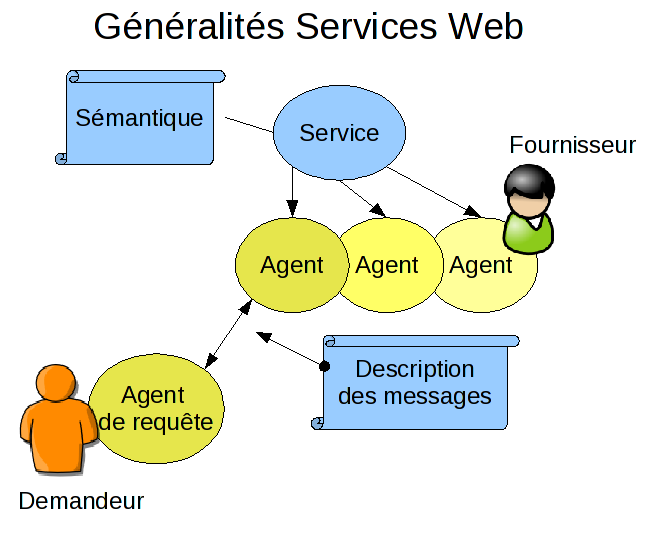
\includegraphics[scale=0.5]{img/Whatisaserviceweb.png}
	\caption{Généralités Services Web}		
	\label{Generalite_figure}
	\centering
\end{figure}						
\newline
Dans la figure \ref{Generalite_figure}, l'agent de requête et l'agent du service utilisent le même format de message, basé sur l'ensemble de standards et de protocoles ouverts déjà existants, tel que le XML.
Ces protocoles sont implémentés par défaut (ou faciles à intégrer) dans la majorité des technologies, ce qui permet la communication entre différentes applications sans contraintes majeures. 
	
Ce système est réalisé grâce à plusieurs technologies, les plus connus étant les services web type SOAP et les services web type REST, détaillés dans les parties 2.5 et 2.6 respectivement.
	

			
\subsection{Caractéristiques d'un Service Web}
Dans un Service Web complet on trouve les caractéristiques suivantes :\cite{refTutorialPointsWS}
\begin{itemize}
	\item Il ne dépend d'aucun système ou langage.
	\item Il est accessible par un réseau (Internet/Intranet).
	\item Il dispose d'une interface publique permettant aux clients d'invoquer des procédures ou méthodes sur des objets distants, l'annuaire du service contient la description de ces fonctionnalités et comment les utiliser.
	\item Utilise un système de messagerie standard (souvent basé sur XML).
	\item Les fonctionnalités utilisées par le service sont regroupées en un nombre limité de \emph{gros grains} qui sont exposés ensuite au client et ainsi permettre une interaction plus simple avec le service. Par exemple, regrouper des fonctions de bas niveau (petites graines) en une seule fonction de haut niveau, et exposer celle-ci sur le réseau.
	\item Son système est \emph{faiblement couplé} : le consommateur de ce service n'est pas directement lié au service. Le service peut changer au fil du temps sans perturber le client, ou peut même disparaitre et le client trouvera un autre service en cherchant dans son annuaire.
\end{itemize}
		
%=================================================================
%=========================== PARTIE HTTP ==========================
%=================================================================
\newpage
\section{Le protocole HTTP}
Avant de passer aux architectures des services web, il est essentiel d'avoir une idée sur le protocole HTTP, qui est le protocole le plus utilisé sur Internet, et donc le plus souvent utilisé dans les architectures décrites dans les sections suivantes.

Dans le modèle client-serveur, les clients et les serveurs échangent des messages dans un modèle de messagerie de type requête-réponse: le client envoie une requête et le serveur renvoie une réponse.
Pour gérer ces messages et définir un format commun entre eux, on utilise le protocole HTTP.

\subsection{HTTP (Hyper Text Transfer Protocol)}
C'est un protocole qui décrit le contenu et la mise en forme des requêtes et des réponses échangées entre le client web et le serveur web. 
Lorsqu'un client, généralement un navigateur web, envoie une requête à un serveur web, il utilise un URL combiné avec un \emph{verbe} HTTP pour spécifier le type de message et l'action que doit prendre le serveur sur une ressource, cette requête est appelée une requête HTTP. Le serveur répond ainsi avec un \emph{réponse HTTP} avec un code HTTP décrivant l'état de la réponse, et le résultat en cas de succès.

\subsection{Méthodes HTTP}
HTTP propose plusieurs verbes (ou méthodes), mais les plus importants sont : 
\begin{itemize}
	\item \textbf{GET} : obtenir des données, un navigateur web envoie une requête GET au serveur web pour demander des pages HTML par exemple.
	\item \textbf{POST} : envoyer des fichiers ou des données vers le serveur web, comme des données de formulaires.
	\item \textbf{PUT} : envoyer des ressources ou du contenu vers le serveur web, similaire à POST mais utilisé principalement pour mettre à jour une ressource, PUT doit être idempotente : c'est-à-dire qu'envoyer plusieurs fois la même requête produit le même résultat que la première.
	\item \textbf{DELETE} : c'est une requête  qui supprime la ressource indiquée.
\end{itemize}

\subsection{HTTPS}
Le protocole HTTP est certes extrêmement flexible, mais il n'est pas sécurisé.
Pour une communication sécurisée via Internet, le protocole HTTPS (HTTP Secure) est utilisé. \newline
Ce protocole utilise le même processus de demande client-réponse serveur que le protocole HTTP, sauf que le flux de données est chiffré avec le protocole SSL (Secure Socket Layer) avant d'être transporté sur le réseau.

\subsection{HTTP/2:}
HTTP/2 est une révision majeure du protocole HTTP, c'est la première nouvelle version de HTTP depuis HTTP 1.1, qui a été standardisé en 1997. Il a été approuvé puis publié en 2015.
Les objectifs principaux de HTTP/2 étaient de rester compatible avec HTTP 1.1 (méthodes, codes HTTP, et les différentes entêtes par exemple), tout en ajoutant de nouvelles fonctionnalités et en diminuant la latence pour ainsi améliorer les temps de chargements de pages web.

%=================================================================
%=========================== PARTIE SOAP ==========================
%=================================================================
\newpage
\section{Services web SOAP} 
\subsection{Le protocole SOAP}
SOAP (Simple Object Access Protocol) est un protocole de communication standardisé par le W3C. 
Il définit un format pour l'envoi des messages (basé sur XML) sous forme d'enveloppe et de son contenu, qui peuvent être envoyées par divers protocoles de transport tel que HTTP et SMTP.
				
SOAP s'appuie donc sur des standards très connus, ce qui lui a donné une grande portabilité et interopérabilité comparée à ses prédécesseurs (COBRA, DCOM, JAVA RMI...etc).
				
\subsection{Structure de message SOAP}
Un message SOAP est un document XML contenant les éléments suivants : \cite{refTutorialPointsSOAP}
\begin{itemize}
	\item \textbf{Enveloppe} : définit le début et fin du message, elle contient contient la spécification des espaces de désignation (namespace\FancyFootNote{Un namespace est un préfixe identifiant de manière unique la signification d'un terme, ou une portion de code en programmation, pour éviter toute ambiguïté.}) et le codage des données. c'est un élément obligatoire.
	\item \textbf{Header (Entête)} : contient des informations ou options supplémentaires pour le traitement du message comme l'encodage, elle est optionnelle.
	\item \textbf{Body (Corps)} : contient les données XML du message à transporter, un élément obligatoire.
	\item \textbf{Fault (Gestion d'erreurs)} : fournit des informations sur les erreurs qui peuvent se produire au traitement de l'information, un élément qui peut être optionnel.
\end{itemize}
\begin{figure}[h]
	\begin{center}
		\includegraphics[scale=1]{img/soapmessagebody.png}
	\end{center}	
	\label{Structure message SOAP}
	\caption{Structure message SOAP}		
	\centering
\end{figure}			
Un message SOAP est un peu lourd, mais reste simple à comprendre et à utiliser. Sa structure offre une fiabilité par rapport au format de données, ainsi qu'un moyen de gérer les erreurs grâce au SOAP Fault.

\subsection{L'architecture orientée services} 
L'architecture orientée services (Service Oriented Architecture, SOA) est style architectural qui vise à concevoir des services web extensibles et hautement réutilisables, et les rendre ensuite visibles et accessibles aux consommateurs.
				
On trouve trois acteurs majeurs dans une architecture SOA de service web :
\begin{itemize}
	\item \textbf{Service Provider} : 
	      c'est le fournisseur du service. Il implémente le service et le rend disponible sur le réseau.
	\item \textbf{Service requester} :
	      c'est le consommateur (client) de ce service. Il utilise un service web existant en ouvrant une connexion réseau et en envoyant des requêtes (par exemple des messages en XML).
	\item \textbf{Annuaire service registry} : 
	      c'est un annuaire de services. Ce registre fournit un endroit central où les développeurs peuvent publier leur nouveau service web, ou trouver d'autres existants.\newline 
\end{itemize}

\begin{figure}[h]
	\center
	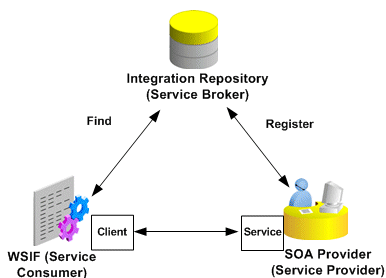
\includegraphics[scale=0.71]{img/SOA.png}
	\caption{Composants d'une architecture orientée services}		
	\centering
\end{figure}		

Les services web emploient un ensemble de technologies qui ont été conçues en respectant une structure en couches sans être dépendantes entre elles. Cette pile, appelée \textbf{Pile de protocoles de services web}, peut évoluer, mais elle est principalement formée de quatre couches : \cite{refTutorialPointsWS}
\begin{description}
	\item[Couche transport] : cette couche est responsable du transport des messages échangés entre les applications. Elle utilise généralement le protocole HTTP, mais d'autres tels que SMTP, FTP ou BEEP peuvent être utilisés.
	\item [Couche communication (Messaging)] : cette couche est responsable de la représentation et formatage des messages échangés entre applications, et ceci afin d'assurer qu'ils soient compris par chaque extrémité. Elle utilise principalement XML (ou un dérivé de ce dernier comme XML-RPC et SOAP), mais peut aussi utiliser d'autres formats standard suivant l'architecture, les services REST peuvent envoyer en simple texte, JSON ou XML par exemple.
	\item[Couche description de service] : cette couche est responsable de la description de l'interface publique du service web, cette description est réalisée en utilisant le WSDL.\newline
	      \texttt{WSDL : (Web Services Description Language)} : c'est un langage de description standard basé sur XML, développé en jointure par Microsoft et IBM. Il permet de décrire différentes informations sur le service web tel que la liste de ses fonctions, comment interagir avec et les invoquer, les ports et protocoles utilisés...etc.
	\item[Couche découverte de service] : cette couche est responsable de centraliser les services dans un registre commun, et fournir des fonctionnalités de recherche/publication de services web. Ce service est assuré par l'annuaire UDDI.\newline
	      \texttt{UDDI (Universal Description, Discovery and Integration)} : c'est un annuaire de services web. Ce protocole, basé sur XML, comporte deux sections en WSDL : les descriptions de ces services et des définitions de ports pour manipuler et rechercher dans l'annuaire.
\end{description}

SOAP est très souvent utilisé avec l'architecture orientée service pour la couche transport et messagerie, combiné avec WSDL et UDDI, on parle de la pile WS-* ( ou \textbf{WS-* stack} en anglais) comme un paradigme ou solution dans la conception de Services Web.

\subsection{Inconvénients}
Bien que SOAP, et plus en général l'architecture SOA, soit une solution standardisée pour la création de Services Web, on peut noter certains inconvénients :
\begin{itemize}
	\item \textbf{Lourdeur:} l'utilisation d'XML et la structure des messages SOAP sont assez verbeuse, XML nécessite aussi d'être parsé\FancyFootNote{Parser XML: Lire le document XML et identifier les fonctions de chaque pièce de ce document, tout en vérifiant sa syntaxe.}, ce qui peut rendre SOAP moins rapide comparé aux autres solutions lorsqu'il nécessite des communications répétées avec le serveur.
	\item \textbf{Limité uniquement à XML:} les messages SOAP et WSDL (XML) sont fortement typés. Bien que ce soit un point fort de XML, ce n'est pas très adapté pour des systèmes faiblement couplés. Changer le moindre paramètre (par exemple, changer un réel en entier) induit un changement de la signature du type et imposera donc à tous les clients de s'adapter.
	\item \textbf{Différents niveaux de support:} on peut trouver SOAP presque automatisé dans certains langages et IDEs (Java, PHP,...etc), mais beaucoup moins supporté dans d'autres, notamment dans les langages au typage dynamique tel que Python et Javascript.
\end{itemize}

En résumé, SOAP et l'architecture qui vient avec sont plus adaptés pour des applications coté entreprises nécessitant une grande robustesse et sécurité sans se soucier des couts engendrés par ce choix.

Ainsi, plusieurs entreprises s'orientent vers REST, et autres ont abandonné leurs services SOAP en faveur de REST, on peut citer comme exemple Google qui a mit fin à son API SOAP en 2009.
\newpage

\section{REST}
Une autre alternative à SOAP et la pile WS-* est REST, un style d'architecture pensée pour être plus proche et plus adapté aux Web. Nous définissons dans cette section ce qu'est REST, les services full-REST et les différents principes qu'ils apportent.

\subsection{Définition}
REST est un terme signifiant \textbf{REpresentational State Transfer}, provenant de la thèse de doctorat de Roy Fielding, publiée en 2000.

REST n'est pas exactement une architecture, mais un ensemble de contraintes qui, lorsqu'elles sont appliquées à la conception d'un système, créent un style architectural logiciel qui délimite les rôles des ressources et des représentations et la façon dont le protocole de transport (souvent HTTP) est utilisé. 
Un serveur qui implémente REST fournit et contrôle l'accès à des ressources (piè 	ces d'information) et les présente aux clients.
			
Un système basé sur REST peut être implémenté dans n'importe quel réseau et architecture disponible en minimisant la complexité de l'implémentation, de la communication et de la distribution.\cite{richardson2008restful}

\subsection{Les ressources}
Une ressource est du contenu identifié par des URI \FancyFootNote{URI (Uniform Resource Identifier): une chaine de caractère servant à identifier une ressource en ayant une certaine hiérarchie, par exemple on peut représenter les livres de catégorie Informatique par "/livre/informatique/"} qui peut être un fichier texte, page HTML, image, vidéos...etc.
REST fournit au client l'accès aux ressources. Il utilise diverses représentations pour représenter une ressource comme le texte, JSON et XML. Aujourd'hui JSON est le format le plus populaire utilisé dans les services REST.

\subsection{Service web full-REST}
Les services web RESTful sont des services web basés sur l'architecture REST, en d'autres termes des services qui respectent les contraintes de REST.
Ces services sont conçus pour fonctionner au mieux sur le web, ils sont légers, maintenables, évolutifs et facilement extensibles et sont donc souvent utilisés pour implémenter des APIs pour des applications web.\cite{refTutorialPointsREST}
\newline 
En résumé, une API est qualifiée de RESTful si elle respecte les critères de REST.
\newline
\newline
\textbf{API Web :} c'est une interface côté serveur qui consiste en un ou plusieurs \emph{points d'entrée} publiques (endpoints) spécifiant la location d'une ressource et comment y accéder, souvent à travers une URI vers laquelle des requêtes (HTTP) sont envoyées, et par laquelle des réponses serveur sont attendues.
Elle définit ainsi un système de requête/réponses entre le client et le serveur à partir de ces points.

\newpage
\subsection{Critères REST}
Une API RESTful complète doit vérifier six (06) critères :
\begin{itemize}
	\item \textbf{Orientée client-serveur}.
	      
	\item \textbf{Sans état} : le serveur ne doit avoir aucune idée de l'état du client entre deux requêtes. Du point de vue du serveur, chaque requête est une entité distincte et indépendante des autres, le service ne devrait donc pas avoir besoin de garder les sessions des utilisateurs.
	      
	\item \textbf{Mise en cache} : un client doit être capable de garder en mémoire des informations sans avoir constamment besoin de demander tout au serveur, tel que les images, polices d'écritures, ...etc.
	      
	\item \textbf{Interface uniforme}: permet à tout composant qui comprend le protocole HTTP d'interagir avec l'application, et avoir la possibilité de modifier l'implémentation côté serveur sans affecter l'interface.
	      
	\item \textbf{Avoir un système de couche}: isolation des différents composants de l'application pour bien organiser leurs responsabilités en prenant en charge leurs éventuelles évolution. Chaque couche représente un système borné qui traite une problématique spécifique de l'application.
	      
	\item \textbf{Fournir un code à la demande: } le serveur peut être capable d'étendre les fonctionnalités d'un client en transmettant une "logique" qu'il peut exécuter, comme des Applets Java ou des scripts en Javascript.
	      
\end{itemize}
Ces contraintes ne dictent pas quel type de technologie utiliser; Ils définissent seulement comment les données sont transférées entre les composants.

\subsection{Architecture}
Dans REST, les interactions entre clients et services sont améliorées par le recours à un nombre limité d'opérations. L'affectation aux ressources de leurs propres identifiants URI uniques autorise une grande souplesse. L'architecture se résume en 5 règles à suivre dans implémentation.\cite{refRegles}
\begin{itemize}
	\item \textbf{Règle 1} : l'URI comme identifiant des ressources.\newline
	      Afin d'identifier une ressource, REST se base sur les URI. Une application se doit construire ses URI (et donc ses URL) de manière précise et statique, en tenant compte des contraintes REST et de futurs changements.
	\item \textbf{Règle 2} : les verbes HTTP comme identifiant des opérations.\newline
	      Utiliser les verbes HTTP existants plutôt que d'inclure l'opération dans l'URI de la ressource. Ainsi, généralement pour une ressource, il y a 4 opérations possibles: Create, Read, Update et Delete, on utilisera les verbes correspondants : POST, GET, PUT et DELETE.
	      Comme chaque verbe possède une signification, REST permet d'éviter toute ambiguïté.
	\item \textbf{Règle 3} : les réponses HTTP comme représentation des ressources.\newline
	      Une ressource peut avoir plusieurs représentations dans des formats divers : HTML, XML, CSV, JSON, etc. C'est au client de définir quel format de réponse il souhaite recevoir via l'entête \emph{Accept} de la requête HTTP, comme il est possible de définir plusieurs formats.
	\item \textbf{Règle 4} : les liens comme relation entre ressources.\newline
	      Les liens d'une ressource vers une indiquent la présence d'une relation. Il est cependant possible de la décrire afin d'améliorer la compréhension du système. Un attribut rel doit être spécifié sur tous les liens.
	\item \textbf{Règle 5 :} un paramètre comme jeton d'authentification.\newline
	      Pour authentifier une requête, les APIs non-triviales utilisent le jeton d'authentification\FancyFootNote{Un jeton est généralement une suite de caractères uniques à l'utilisateur, par laquelle le serveur peut identifier et ainsi authentifier ses requêtes}. Chaque requête est envoyée avec un jeton passé en paramètre ou dans l'entête. Ce jeton temporaire peut être obtenu en envoyant une première requête authentification puis en le combinant avec les requêtes suivantes.
\end{itemize}
\subsection{Le format JSON}
JSON (JavaScript Object Notation) est un format léger d'échange de données. Il est basé sur un sous-ensemble du langage de programmation. C’est un format texte indépendant de tout langage.
Ces propriétés font de lui un langage d'échange de données idéales, qui est facile à lire ou à écrire pour des humains. Il est aisément analysable ou générable par des machines. 
JSON se base sur deux structures:
\begin{itemize}
	
	\item Une collection de couples nom/valeur. 
	\item Une liste de valeurs ordonnée. 
\end{itemize}
Ces structures prennent les formes suivantes :
\begin{itemize}
	\item Un objet, qui est un ensemble de couples nom/valeur non ordonnés. 
	\item Un tableau est une collection de valeurs ordonnées. 
	\item Une valeur peut être soit une chaîne de caractères entre guillemets, un nombre, un booléen, un objet ou un tableau. Ces structures peuvent être imbriquées.
	      
\end{itemize}

\lstset{style=JSON}

\begin{figure}[h!]
  \centering
  \begin{subfigure}[b]{0.52\linewidth}
      \begin{lstlisting}[caption=Exemple en XML]
<?xml version="1.0" encoding="UTF-8"?>
<root>
  <fleuves>
     <fleuve>
       <continent>Asie</continent>
         <embouchure>
          Mer de Laptev
         </embouchure>
         <longueur>4400</longueur>
         <nom>Lena</nom>
    </fleuve>
    ...
  </fleuves>
</root>
\end{lstlisting}
  \end{subfigure}\hfill%  
  \begin{subfigure}[b]{0.40\linewidth}
      \begin{lstlisting}[caption=Equivalent en JSON]
{
  "fleuves":
  [
    {
      "nom": "Lena",
      "longueur": "4400",
      "continent": "Asie",
      "embouchure": "Mer de Laptev"
    },
    ...
  ]
}       
\end{lstlisting}
\end{subfigure}\hfill%
\caption{Exemples de données en XML et JSON.}
\end{figure}


\subsection{Avantages}
REST devient de plus en plus utilisé dans les entreprises aujourd'hui, les principales motivations pour ce choix sont:\cite{refSOAPvsREST}
\begin{itemize}
	\item Plus grande simplicité d'implémentation, aucun besoin d'outils pour interagir avec.
	\item Courbe d'apprentissage plus petite pour les développeurs.
	\item Utilisation de multiples formats pour l'échange de données (XML, JSON, HTML), notamment le format JSON qui est plus léger que HTML et plus adapté à certains langages (comme Javascript).
	\item Plus proche de la conception et de la philosophie initiale du Web (URI, GET, POST, PUT et DELETE).
	\item Pas de gestion d'états du client sur le serveur.
	\item Favorise la compatibilité au niveau de la couche de présentation.
	\item Peut être implémenté localement.
	\item Utilise l'URI comme représentation de ses ressources, ce qui lui donne une flexibilité d'évolution (changer l'implémentation sans changer l'URL et donc sans affecter le client).
\end{itemize}
\subsection{Limites}
\begin{itemize}
	\item Difficile de respecter l'autorisation et la sécurité
	\item Ne convient pas pour gérer une grande quantité de données
	\item Moins sécurisé comparé à SOAP
	\item Il est sans état
	\item Ne peut pas être utilisé lorsque les interactions client et serveur sont essentielles
	\item Ne peut pas être utilisé pour les transactions impliquant plusieurs appels
\end{itemize}
\subsection{REST vs SOAP}
** points à mentionner : 
\begin{itemize}
	\item expliquer que REST est un style architectural, SOAP un protocole
	\item REST n'est pas lié à XML contrairement à SOAP
	\item SOAP est strictement typé et a une spécification standard plus stricte pendant que REST donne le concept et est moins restreint dans l'implementation 
	\item SOAP a une gestion des erreurs par défaut ( vu dans son enveloppe ), expliquer utilité pour un exemple de transaction bancaire
\end{itemize}				 
			
(a faire) conclusion : SOAP peut être utile pour des applications d'entreprises demandant une haute sécurité "unless you have a good reason, use REST" 
\section{Exemples et applications}
Deux-Trois Api connues, exemple avec Google Maps
\section{XML-RPC, gRPG et GraphQL}
\begin{description}
\item[XML-RPC:] c'est un protocole RPC
 \FancyFootNote{\textbf{RPC }(Remote Procedure Call): c'est un protocole qu'un programme peut utiliser pour demander un service d'un autre programme situé dans une machine distante sans avoir à comprendre son système de façon similaire à un appel de fonction locale.}
qui utilise XML pour encoder ses messages et les envoyer, généralement, par HTTP.
C'est une deuxième manière plus simple d'implémenter RPC en utilisant XML, SOAP étant la première. Nous ne considérons pas ce protocole car malgré sa simplicité, il est moins flexible nécessitant une dépendance étroite entre le client et serveur, contrairement aux clients REST qui sont \emph{faiblement couplés}.

Il existe aussi JSON-RPC qui est similaire à XML-RPC.

\item[gRPC: ] c'est un framework RPC initialement développé par Google. Il utilise le protocole HTTP/2 pour le transport, Protocol Buffers comme langage de description d'interface, et offre plusieurs fonctionnalités telles que l'authentification, Il permet la construction de liaisons client/serveur multiplateforme pour de nombreux langages.
Nous n'avons pas considéré d'utiliser gRPC du fait qu'il soit encore nouveau au moment d'écrire ce rapport, mais aussi parce qu'il est plus adapté pour des architectures en \emph{micro-services}.

\item[GraphQL:] c'est un langage de requête open-source pour les APIs, une spécification sur comment satisfaire ces requêtes avec les données existantes ainsi qu'une description complète et fortement typé de toutes les données de l'API.
Développé initialement par Facebook en 2012, et finalement publié en 2016, son langage de requête permet au client de consulter la description complète des ressources, et de demander exactement les données dont il a besoin en une seule requête, et donc sans avoir à faire plusieurs requêtes avec le serveur ni avoir à récupérer des attributs en plus, ce qui est un des inconvénients de REST.
Cette technologie est encore nouvelle au moment d'écrire ce rapport, mais promet d'être un bon remplaçant de REST.


La technologie reste nouvelle, son implémentation n'est donc pas très bien supportée et ses avantages ne sont pas très signifiants pour notre application, nous avons donc choisi de la laisser comme perspective. 
De plus, GraphQL peut être ajouté comme une couche supplémentaire sur une ou plusieurs APIs, ce qui rend possible d'implémenter une API GraphQL au dessus de notre API REST dans de futures version sans avoir à modifier ou écraser l'implémentation courante.
\end{description}

\section{Conclusion : pourquoi choisir REST}
	Après avoir exploré les différentes technologies, nous avons choisi d'implémenter notre Service Web en utilisant REST qui est plus simple à mettre au point mais aussi plus flexible que SOAP, ce qui permettra d'améliorer et faire évoluer ensuite ce projet plus rapidement.
	
	Il existe encore certains principes qui n'ont pas été cités dans ce chapitre, bien qu'il n'existe pas réellement une manière absolue pour implémenter une API REST, il existe certaines \emph{bonnes pratiques} que nous tâcherons d'implémenter dans ce projet. Le résultat ainsi que les détails d'implémentation seront décrits dans les chapitres suivants.
